% Figura cuerpo B2 (3.4.2): perturbación de costes: el menú de la disyuntiva
\documentclass[tikz,border=3pt]{standalone}
\usepackage[T1]{fontenc}
\usepackage[utf8]{inputenc}
\usepackage{amsmath}
\usetikzlibrary{arrows.meta,calc,positioning}
\begin{document}
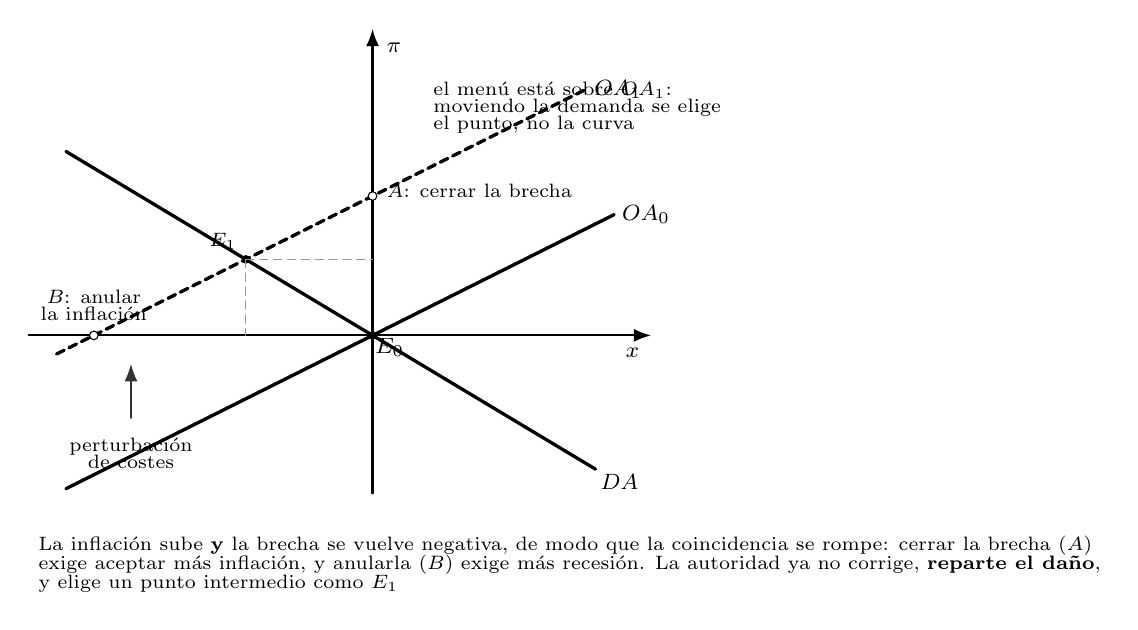
\begin{tikzpicture}[>={Latex[length=2.2mm]}, line cap=round, font=\footnotesize, scale=1.18,
  eje/.style={->, thick},
  curva/.style={very thick},
  nueva/.style={very thick, densely dashed},
  guia/.style={densely dashed, gray!80},
  pto/.style={circle, fill=black, inner sep=1.1pt},
  contra/.style={circle, draw=black, fill=white, inner sep=1.1pt}]

  \draw[eje] (-3.7,0) -- (3.0,0) node[below left=1pt]{$x$};
  \draw[eje] (0,-1.7) -- (0,3.3) node[below right=2pt]{$\pi$};

  \draw[curva] (-3.3,-1.65) -- (2.6,1.30) node[right=-1pt]{$OA_{0}$};
  \draw[nueva] (-3.4,-0.20) -- (2.3,2.65) node[right=-1pt]{$OA_{1}$};
  \draw[curva] (-3.3,1.98) -- (2.4,-1.44) node[below right=-3pt]{$DA$};

  \draw[->, gray!40!black, shorten >=2pt, shorten <=2pt] (-2.6,-0.95) -- (-2.6,-0.25);
  \node[anchor=north, font=\scriptsize, align=center] at (-2.6,-1.00) {perturbación\\[-2pt]de costes};

  \node[pto] (E0) at (0,0) {};
  \node[below right=-2pt of E0, inner sep=1pt] {$E_{0}$};
  \node[contra] (A) at (0,1.5) {};
  \node[anchor=west, inner sep=3pt, font=\scriptsize] at (0.06,1.56) {$A$: cerrar la brecha};
  \node[contra] (B) at (-3.0,0) {};
  \node[anchor=south, inner sep=2pt, font=\scriptsize, align=center] at (-3.0,0.10) {$B$: anular\\[-2pt]la inflación};
  \node[pto] (E1) at (-1.364,0.818) {};
  \node[anchor=south east, inner sep=2pt, font=\scriptsize] at (-1.40,0.86) {$E_{1}$};

  \draw[guia] (-1.364,0.818) -- (-1.364,0);
  \draw[guia] (-1.364,0.818) -- (0,0.818);

  \node[anchor=west, font=\scriptsize, align=left] at (0.55,2.45) {el menú está sobre $OA_{1}$:\\[-2pt]moviendo la demanda se elige\\[-2pt]el punto, no la curva};

  \node[align=left, anchor=north west, font=\scriptsize] at (-3.7,-2.05)
    {La inflación sube \textbf{y} la brecha se vuelve negativa, de modo que la coincidencia se rompe: cerrar la brecha ($A$)\\[-1pt]exige aceptar más inflación, y anularla ($B$) exige más recesión. La autoridad ya no corrige, \textbf{reparte el daño},\\[-1pt]y elige un punto intermedio como $E_{1}$};
\end{tikzpicture}
\end{document}
